\section{Simulering}

I dette afsnit laves simuleringen for det samlede kredsløb i 2. iteration. 
Selve simuleringsdokumentet er delt op i blokke for at gøre det mere overskueligt. 


\noindent Kigges der på det yderste trin på figur~\ref{fig: simtop}, ses blot indgangsspændingen på 26V og udgangsloaden, der er sat op til $8.4\ohm$.
\begin{figure}[H]
	\center
	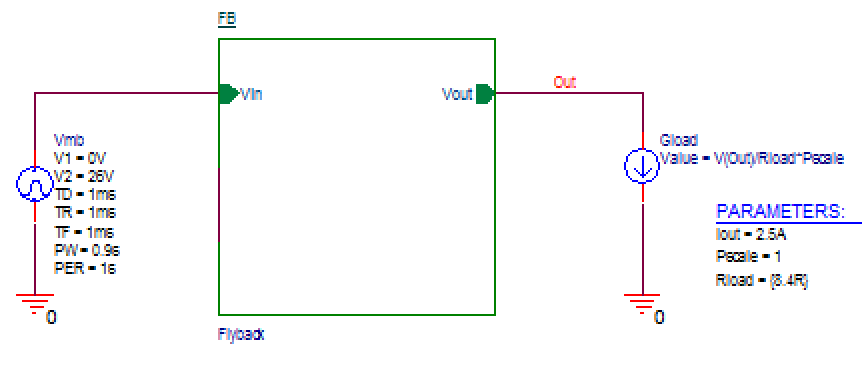
\includegraphics[max width=0.7\linewidth]{/tex/2iteration/billeder/Simulering_2iteration_top.png}
	\caption{Yderste blok af simulering}
	\label{fig: simtop}
\end{figure}
Imellem er blokken "Flyback". Heri er selve kredsløbet. Dykkes der ind i denne blok fås det der ses på figur~\ref{fig: simfly} 
\begin{figure}[H]
	\center
	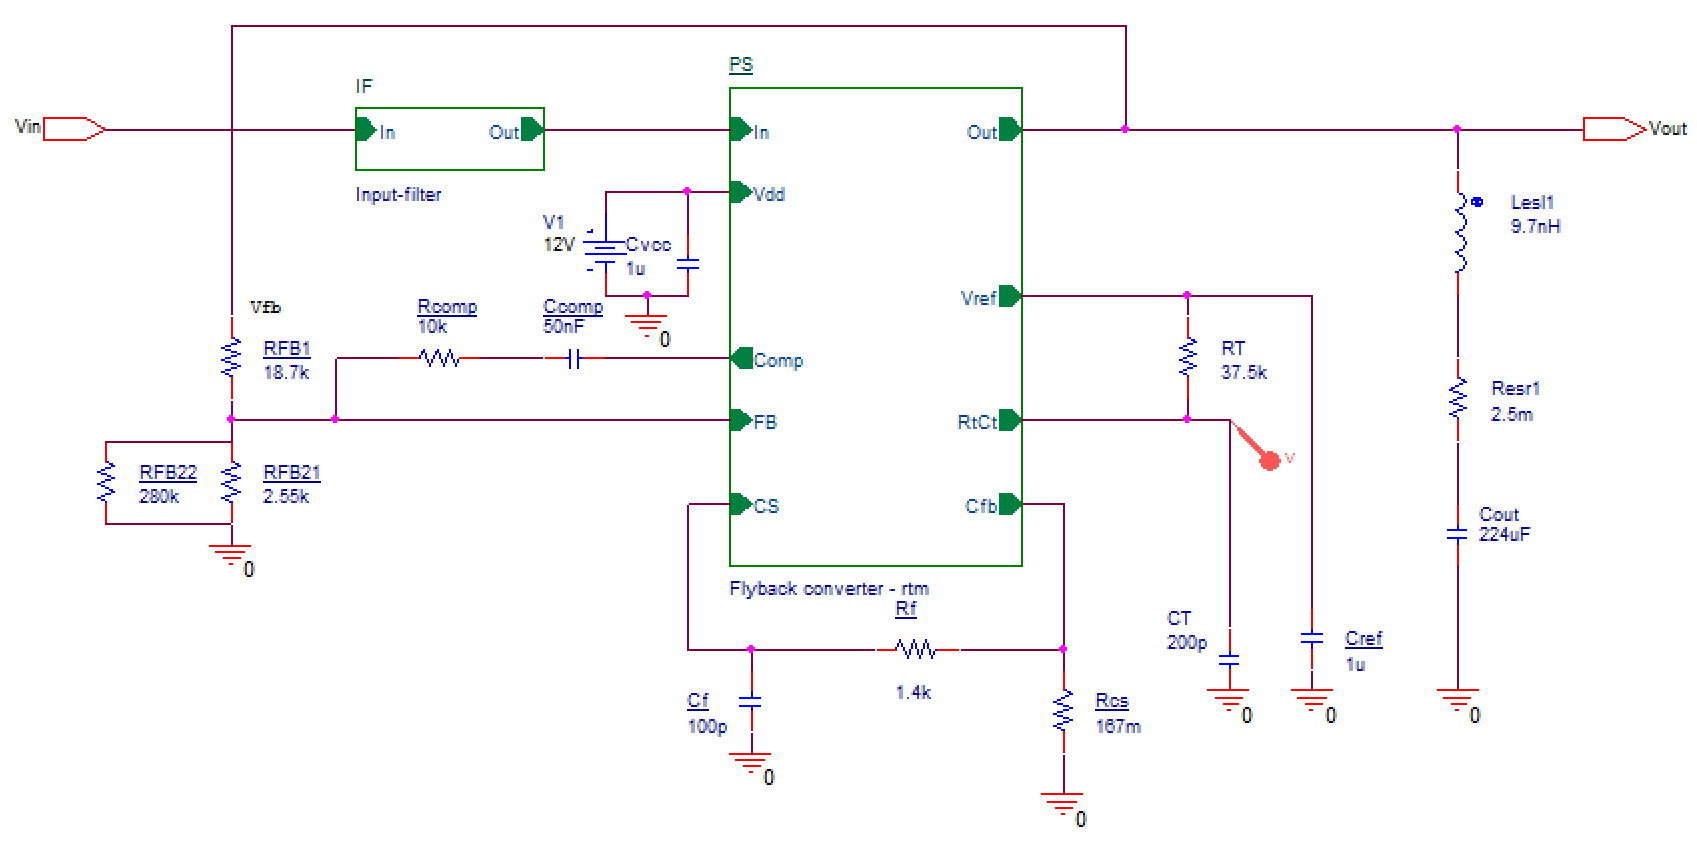
\includegraphics[max width=0.7\linewidth]{/tex/2iteration/billeder/Simulering_2iteration_flyback.png}
	\caption{Flyback blok}
	\label{fig: simfly}
\end{figure}
Her ses yderligere 2 blokke hhv. Inputfilter og flyback converter. Ud over disse blokke ses de komponenter, der er brugt til at få PWM controlleren til at køre efter hensigten. Selve controlleren ligger inde i flyback converter blokken. Værdierne og forklaringen af komponenterne blev gennemgået i analyse afsnittet om PWM controlleren??
Desuden ses output kondensatoren med de udregnede parasitter også.


\noindent Blokken for inputfiltret er allerede vist tidligere under forklaringen af denne, så den vises ikke igen. Til gengæld ses indholdet af Flyback converter blokken på figur~\ref{fig: simflycon}. 
\begin{figure}[H]
	\center
	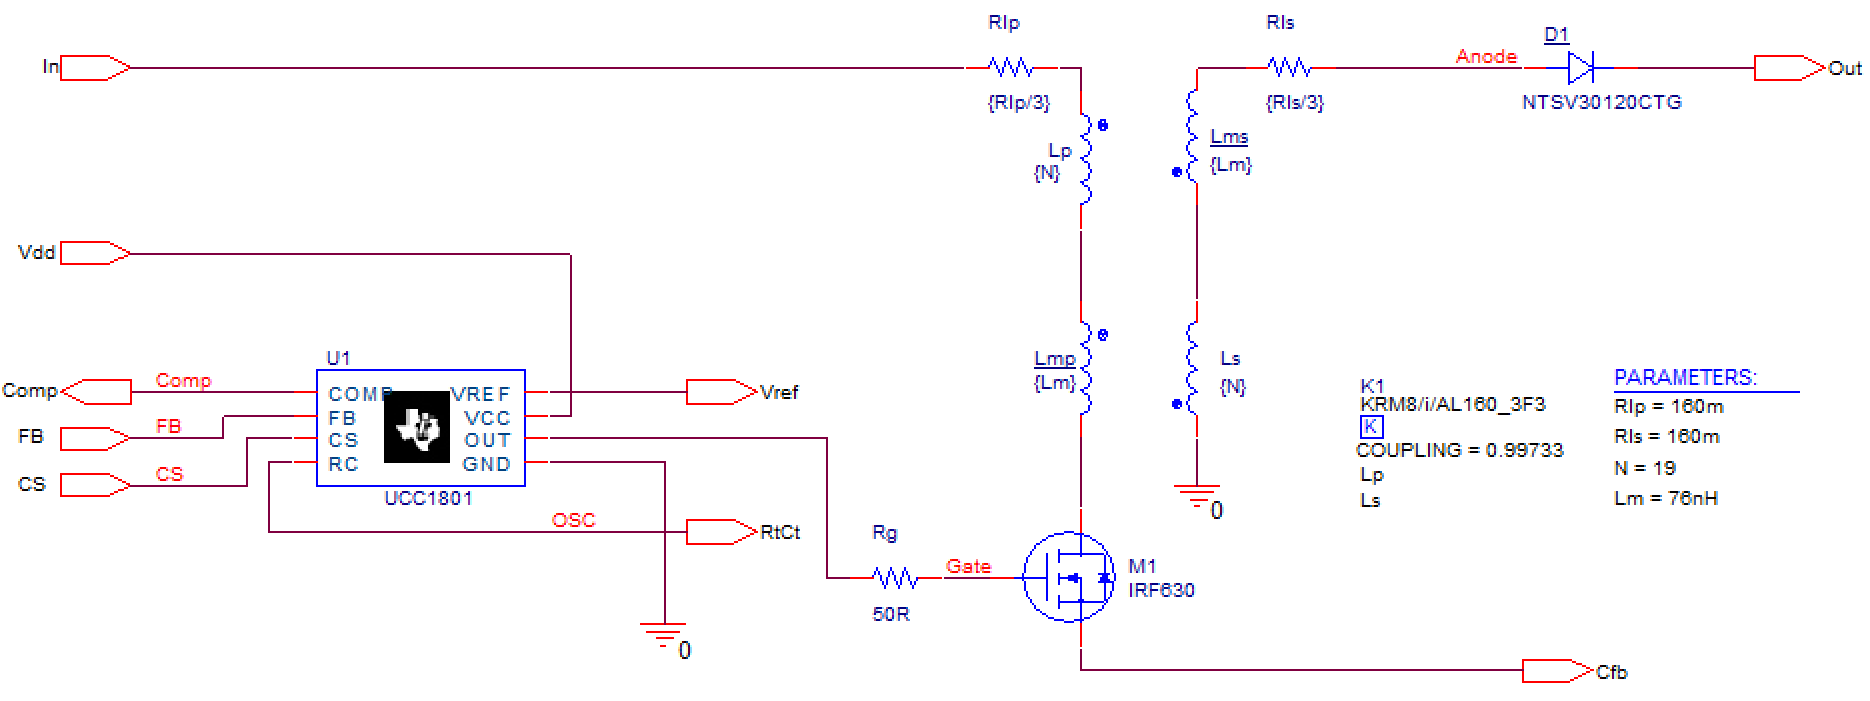
\includegraphics[max width=0.7\linewidth]{/tex/2iteration/billeder/Simulering_2iteration_flycon.png}
	\caption{Flyback converter blok}
	\label{fig: simflycon}
\end{figure}
Heri ses selve PWM controlleren UCC1801, som der er trukket en model ind for. \cite{??}. Også MOSFET'en og Dioden er der trukket modeller ind for. Ved MOSFET'en har det ikke været muligt at finde den præcise model. Derfor er IRF630 modellen istedet brugt, da det er vurderet, at den minder en del om den\cite{IRF630}. 
Yderligere ses transformatoren, hvor både spredningsselvinduktion og kobbermodstanden i ledningerne er tegnet med samt kernemodellen for 3F3 er trukket ind.

%%% Simulering af PWM-controller for 2. iteration

\subsection{PWM-controller}
I det følgende afsnit simuleres funktionaliteterne omkring PWM-controlleren. Her simuleres frekvensen af savtandspændingen og selve switch-frekvensen, samt signalet over current-sense modstanden både før og efter filteret.

\subsubsection{Switch-frekvens}
\noindent Først simuleres frekvensen af savtandspændingen. Dette er gjort på figur~\ref{fig:Simulering_PWM_savtand}. Periodetiden af savtandspændingen aflæses til $5.01\micro s$. Omregnet til en frekvens giver det: $f_{osc}=\frac{1}{5.01\micro s}=199.6k\hertz$. Derudover aflæses signalets minimumsspænding til ca. $138mV$, og maksimum- til ca. $2.5V$. I følge teorien burde spændingen ligge mellem $200mV$ og $2.65V$.

\begin{figure}[H]
	\center
	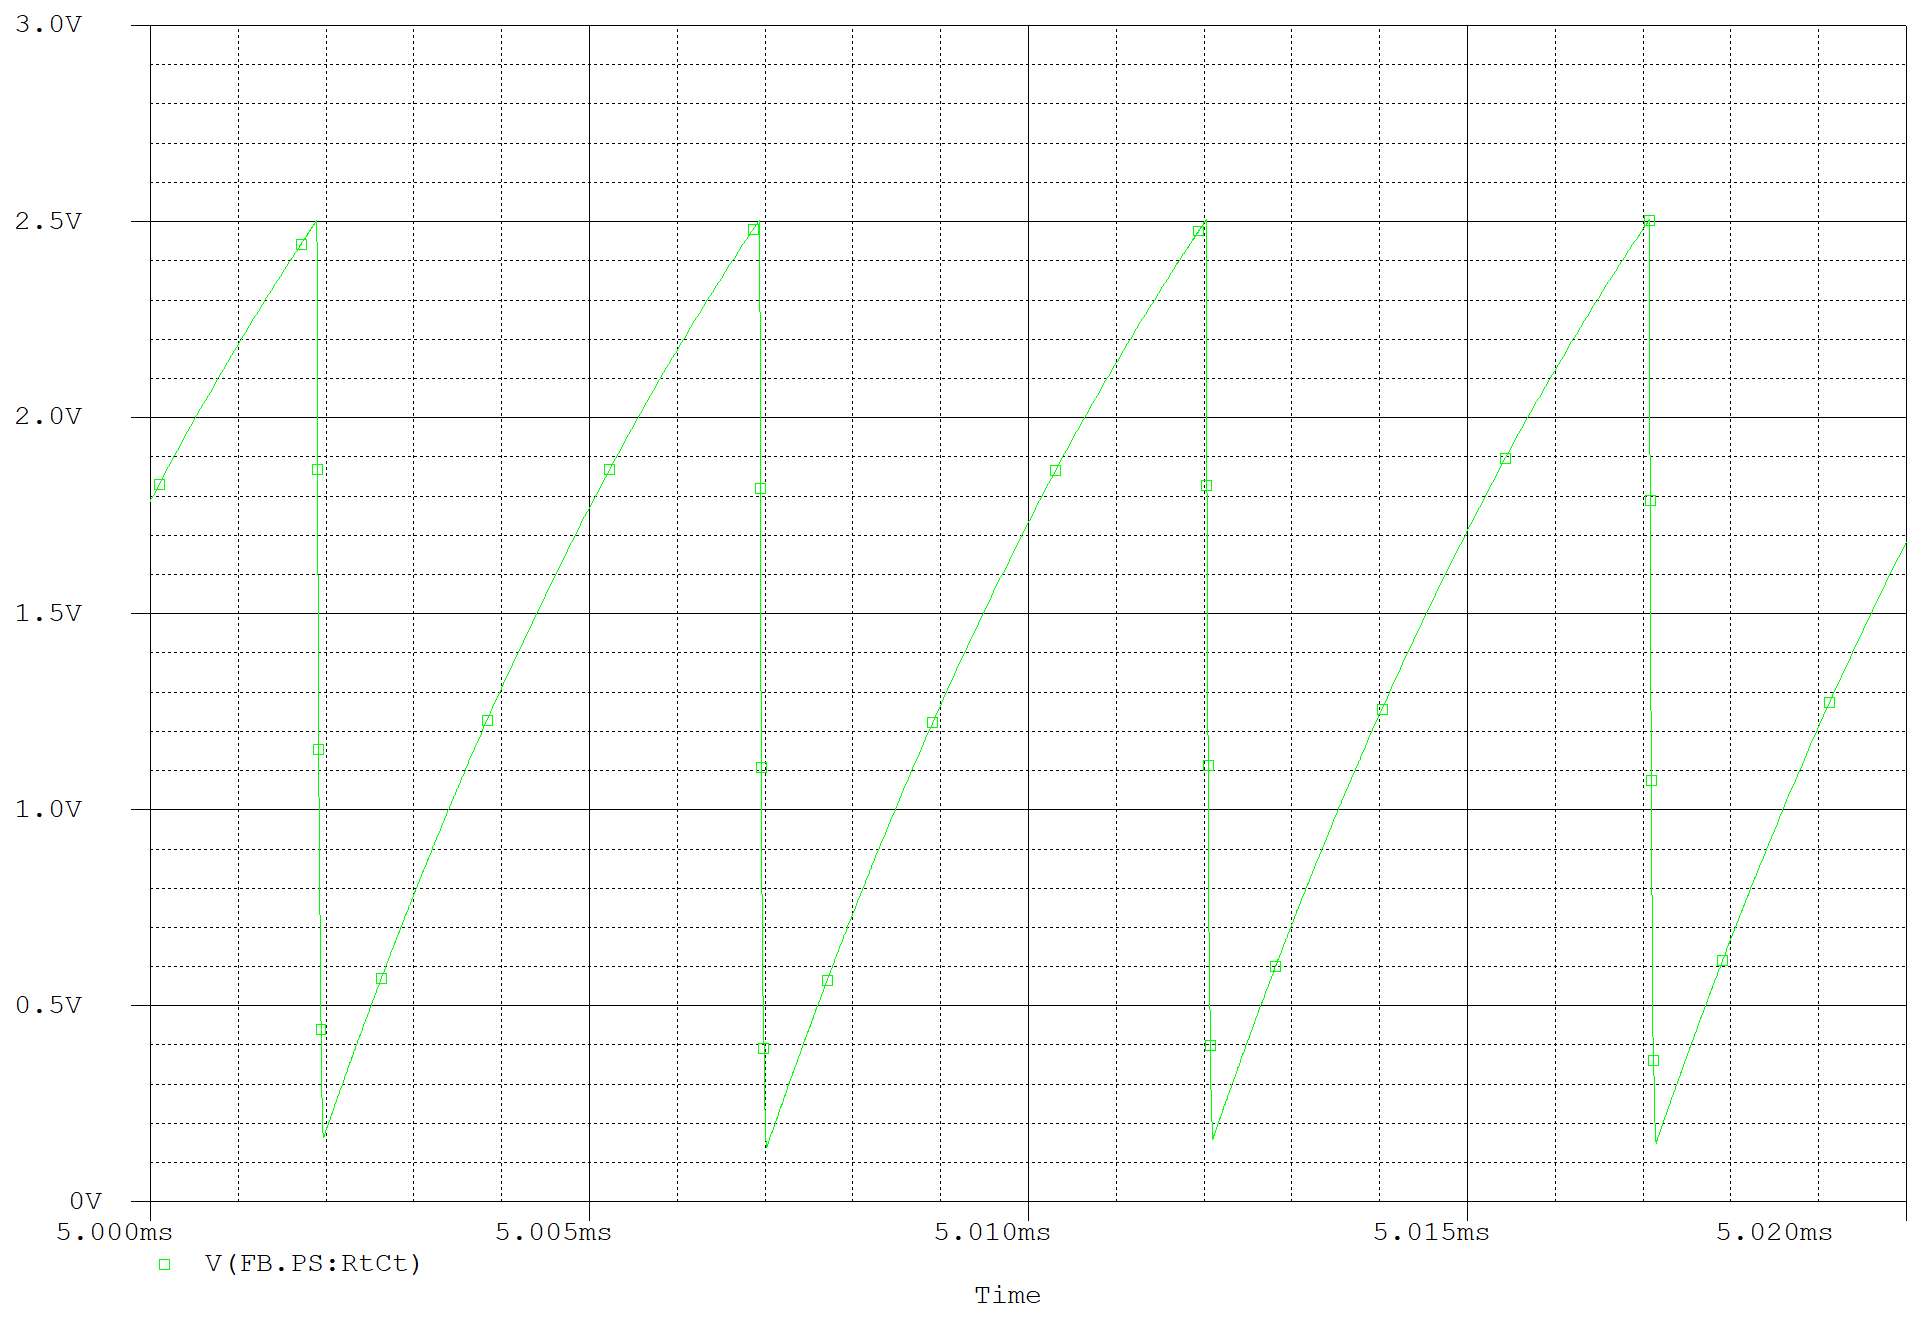
\includegraphics[max width=0.9\linewidth]{/tex/2iteration/billeder/Simulering_PWM_savtand.png}
	\caption{Simulering af savtandspændingen}
	\label{fig:Simulering_PWM_savtand}
\end{figure}

\noindent Nu simuleres selve switch-frekvensen. Dette er gjort på figur~\ref{fig:Simulering_PWM_switch_frekvens}, hvor der måles på udgangen af PWM-controlleren. Her måles periodetiden til $10.1\micro s$, eller en frekvens på $f_s=99.01k\hertz$. 

\begin{figure}[H]
	\center
	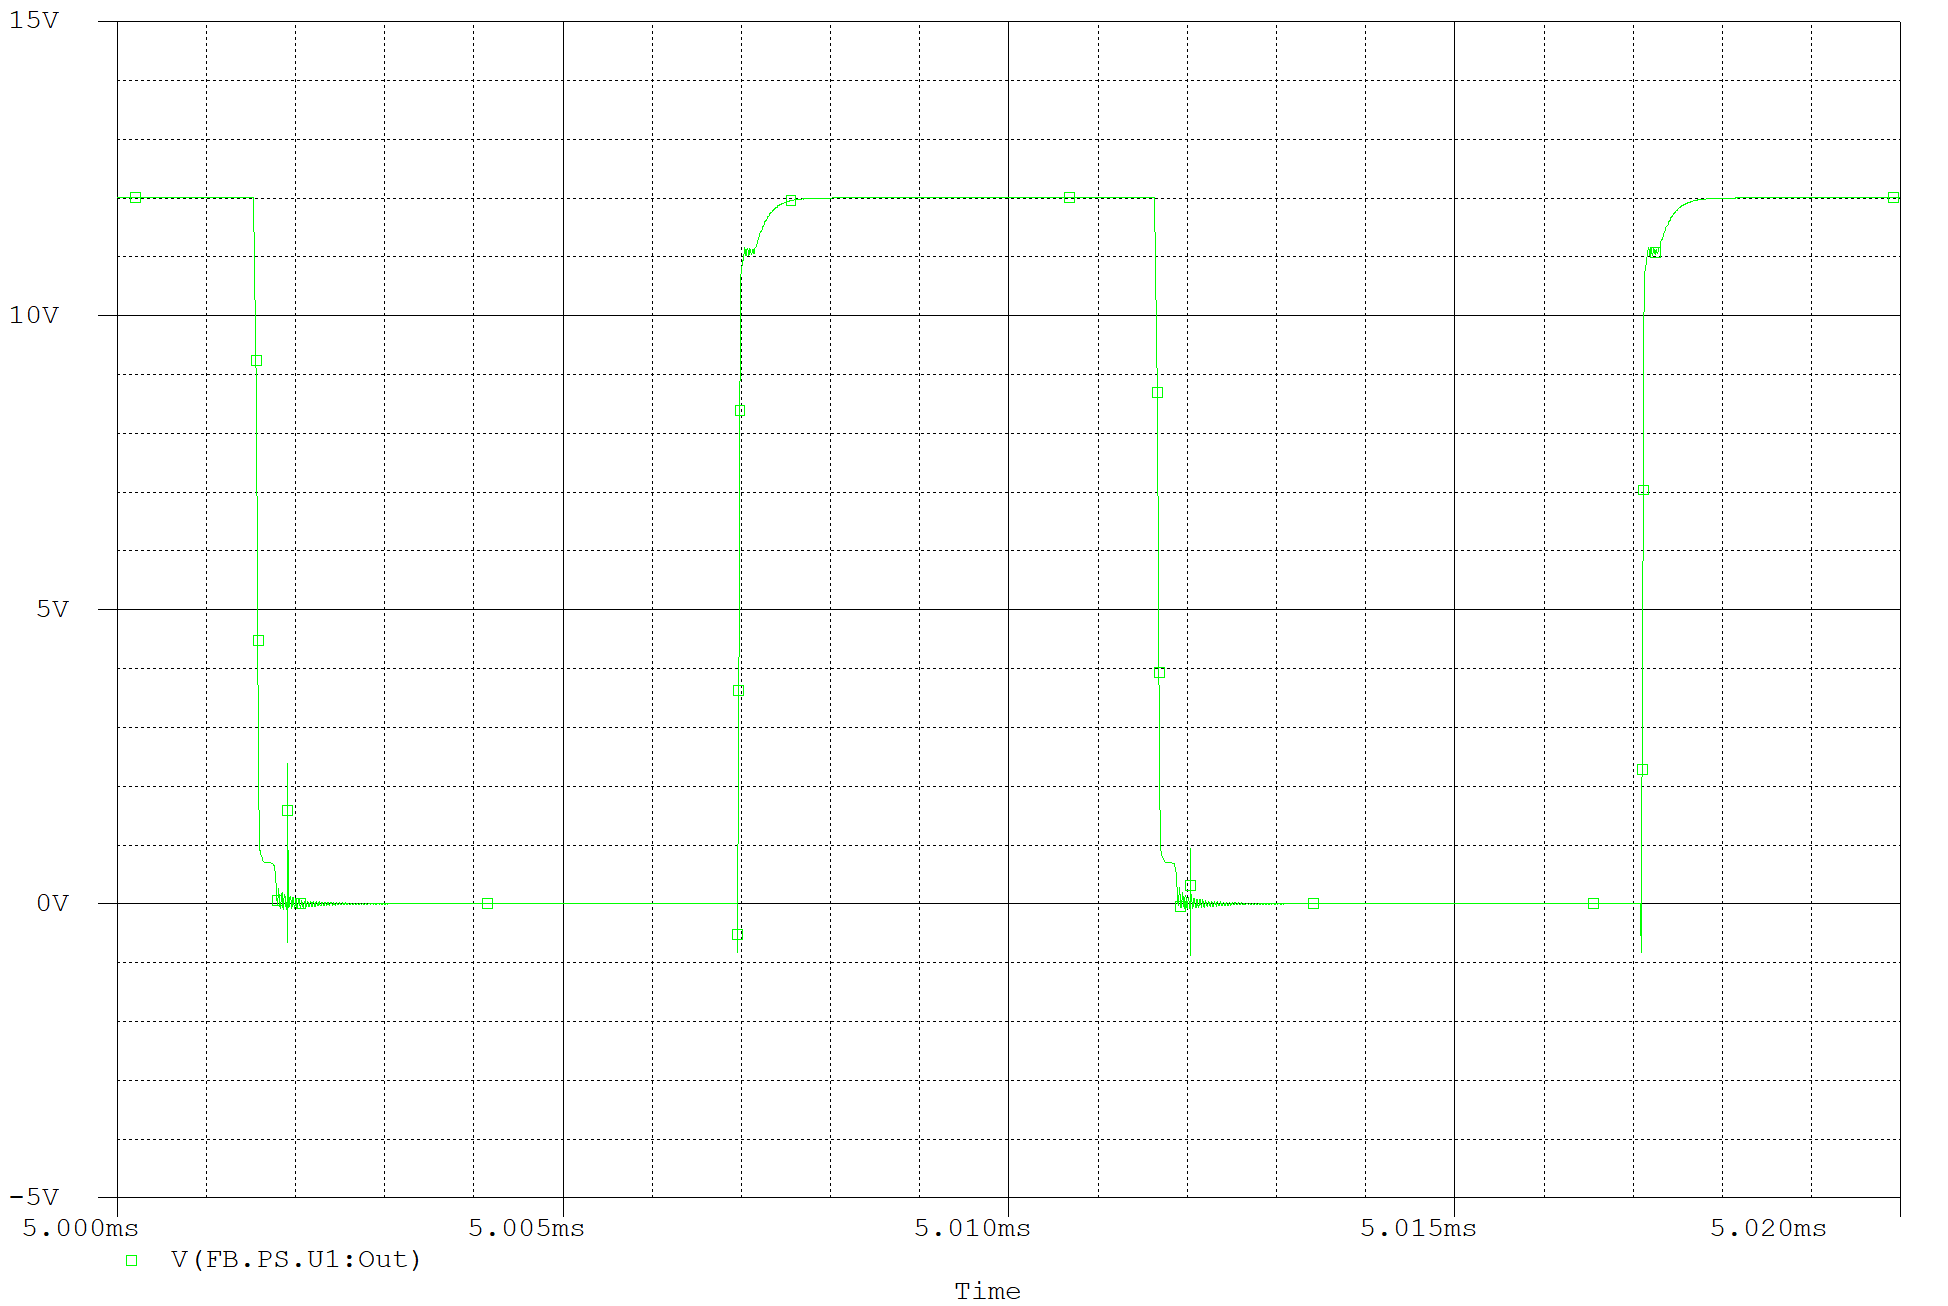
\includegraphics[max width=0.9\linewidth]{/tex/2iteration/billeder/Simulering_PWM_switch_frekvens.png}
	\caption{Simulering af switch-frekvens}
	\label{fig:Simulering_PWM_switch_frekvens}
\end{figure}

\subsubsection{Switch-tid}
\noindent Simuleringen af switch-tiden i MOSFET'en er vist på figur~\ref{fig:Simulering_MOSFET_switch_tid}. Figuren viser et zoom af MOSFET'ens gate signal. Switch-tiden kan aflæses som tiden af signalets plateau. Det aflæses til ca. $103ns$. Grunden til dette afviger meget fra analysen, er modellen for den MOSFET der bruges i simuleringen. Som nævnt bruges en anden MOSFET i simuleringen, end der er regnet med i analysen. En af de specifikationer de afviger mellem de to MOSFETs er \textit{Miller} ladningen, der bruges til at regne switch-tiden. I databladet for IRF630\cite{IRF630}, aflæses den til $15nC$. Regnes switch-tiden ud fra det, fås $107.1ns$, hvilket stemmer med det simulerede. 
\begin{equation} 
T_{ch} = \frac{Q_{gd} \cdot R_{g}}{V_{DD}-V_{gs}} = \frac{15nC \cdot 50\ohm}{12V-5V} = 107.1ns
\end{equation}

\begin{figure}[H]
	\center
	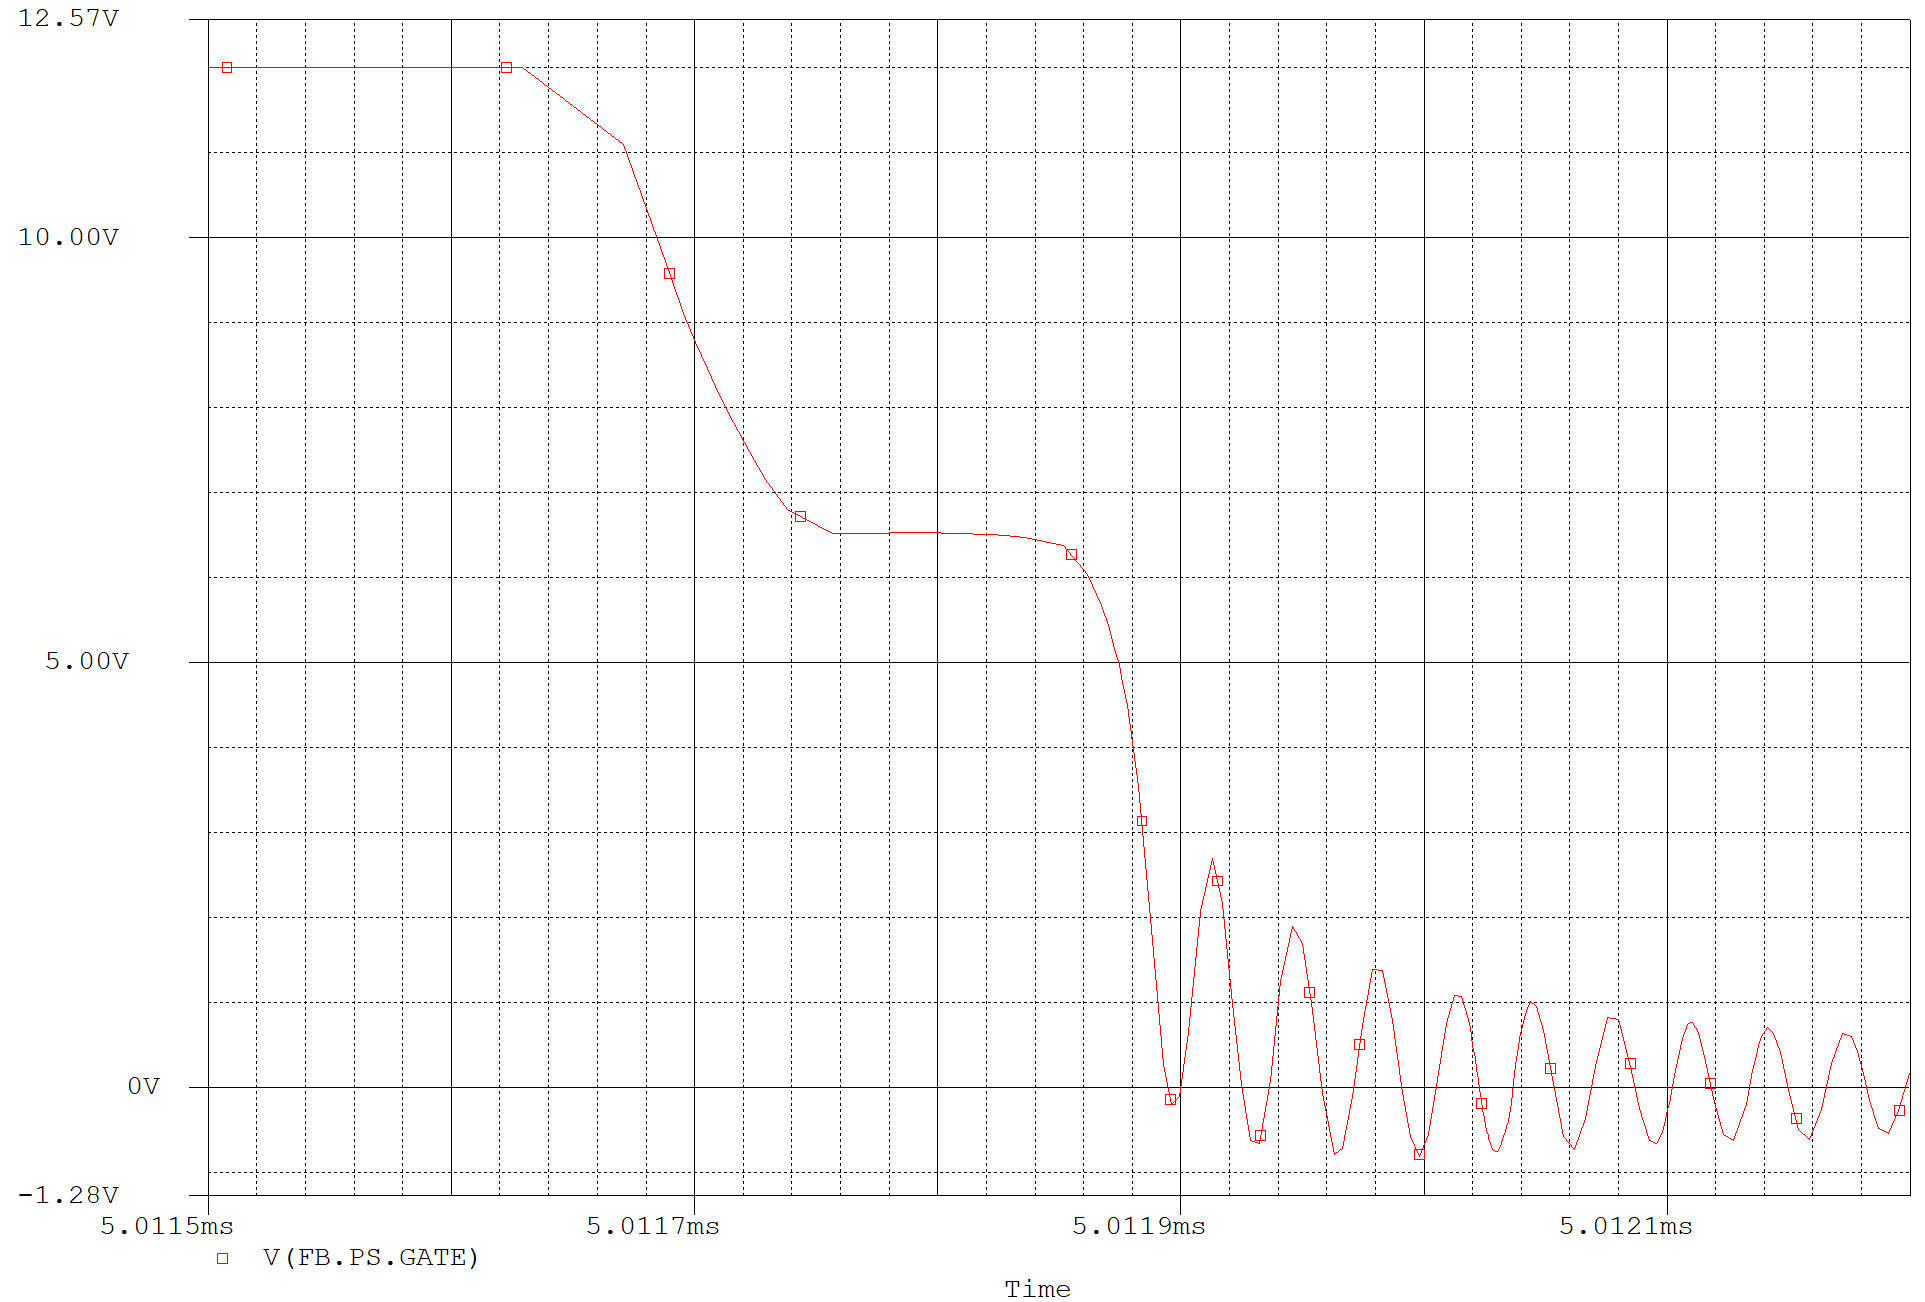
\includegraphics[max width=0.9\linewidth]{/tex/2iteration/billeder/Simulering_MOSFET_switch_tid.png}
	\caption{Simulering af switch-tid i MOSFET}
	\label{fig:Simulering_MOSFET_switch_tid}
\end{figure}


\subsubsection{Current-sense}
\noindent Current-sense signalet måles både før og efter filtreringen. Signalet før filteret ses på figur~\ref{fig:Simulering_PWM_current_sense_U}. Her ses de spikes på signalet, der kan give anledning til en forkert duty-cycle. Figur~\ref{fig:Simulering_PWM_current_sense_M} viser simuleringen for signalet efter filtreringen. Her ses det, at spikesene er blevet filtreret væk, dog med den konsekvens at signalet har fået en langsommere stigetid. Stigetiden aflæses til ca. $280ns$. Ifølge teorien burde PWM-controllerens udgangssignal skifte, når current-sense signalet er lig $1V$. På figur~\ref{fig:Simulering_PWM_current_sense_M}, ses det, at dette også er tilfældet for p-spice modellen for UCC1801. 


\begin{figure}[H]
	\center
	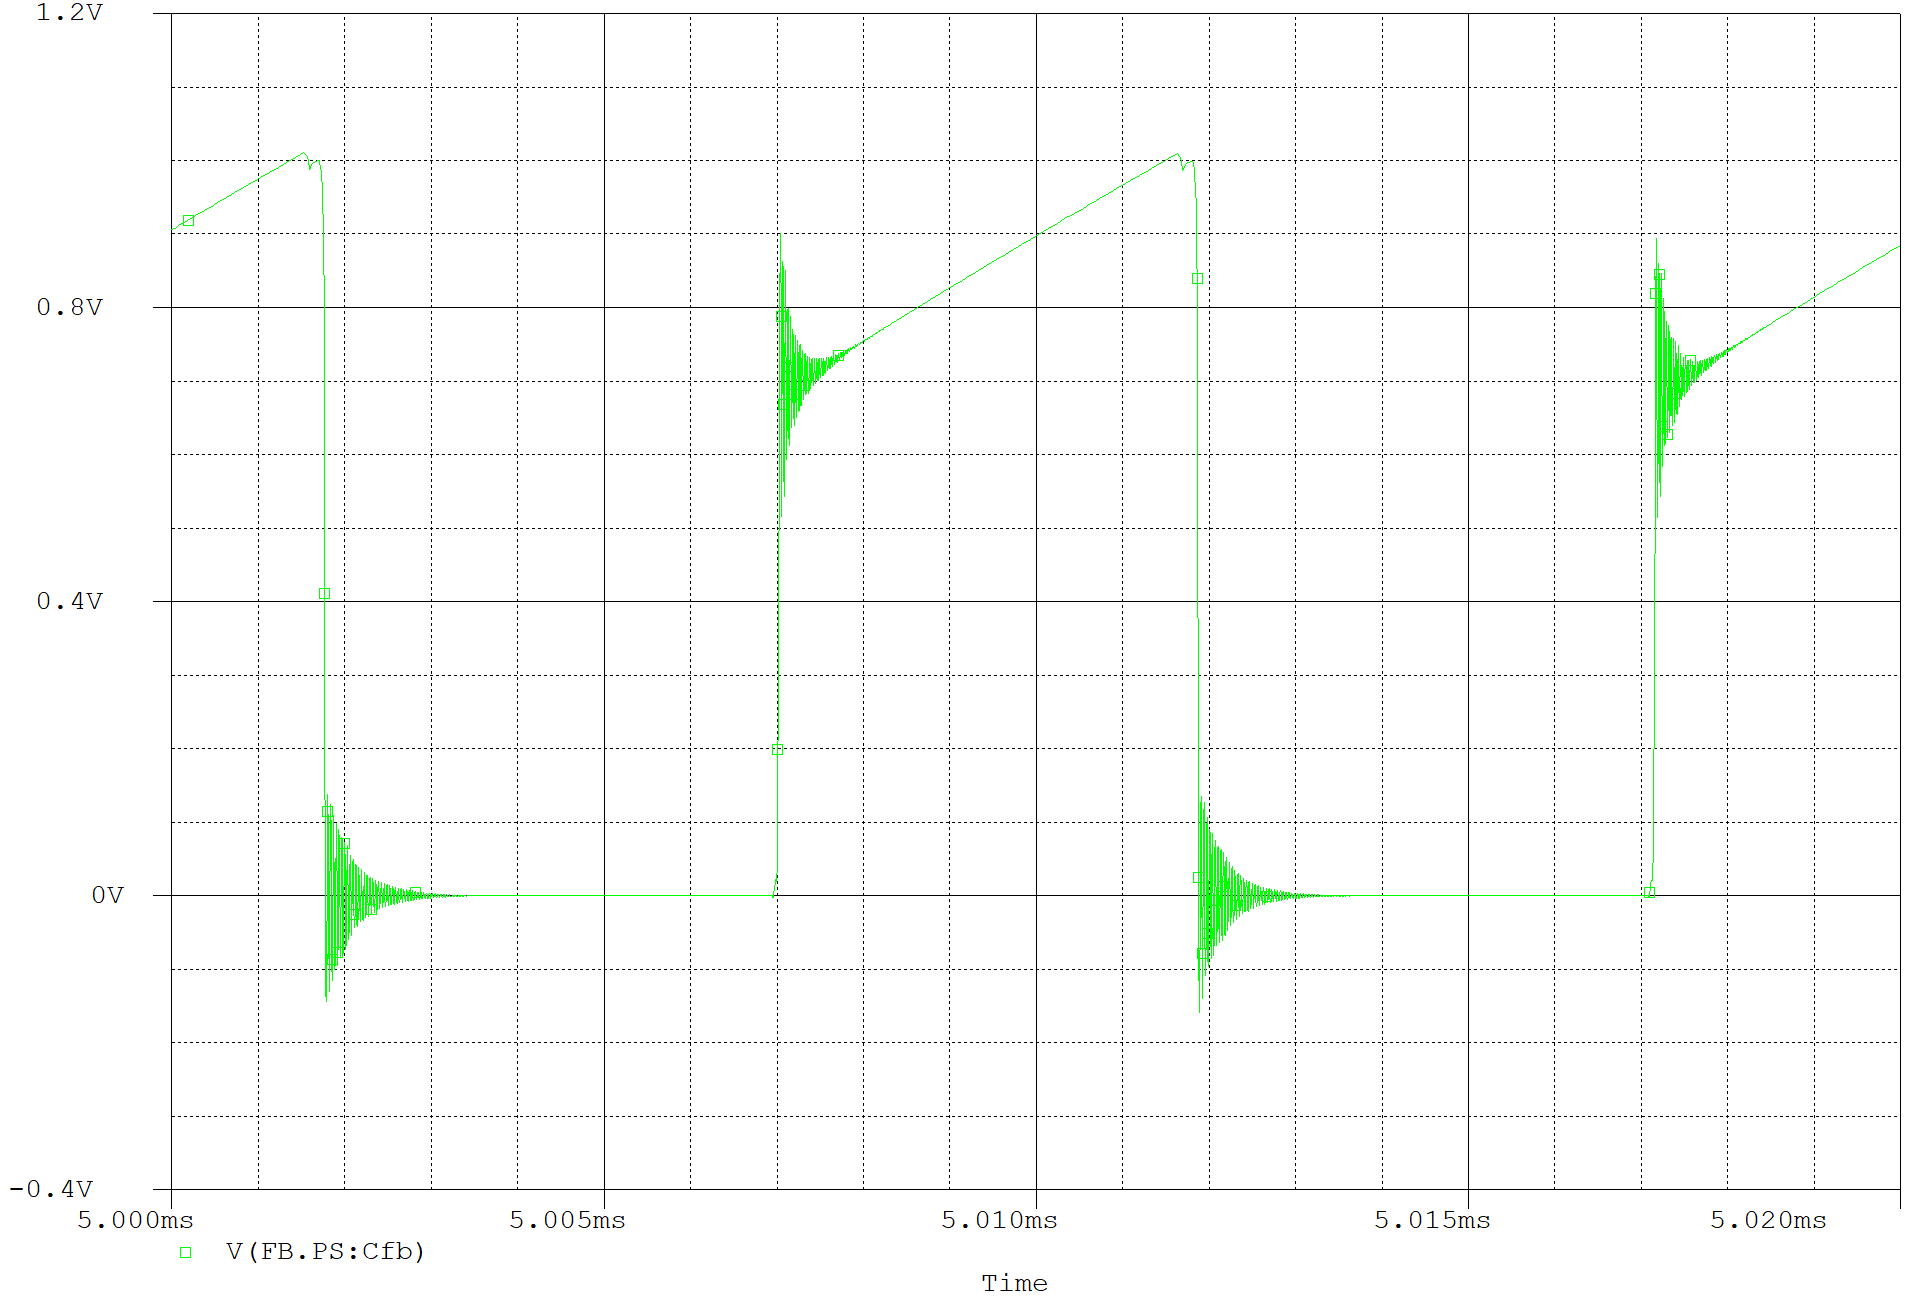
\includegraphics[max width=0.9\linewidth]{/tex/2iteration/billeder/Simulering_PWM_current_sense_U.png}
	\caption{Simulering af current-sense signal før filtrering}
	\label{fig:Simulering_PWM_current_sense_U}
\end{figure}

\begin{figure}[H]
	\center
	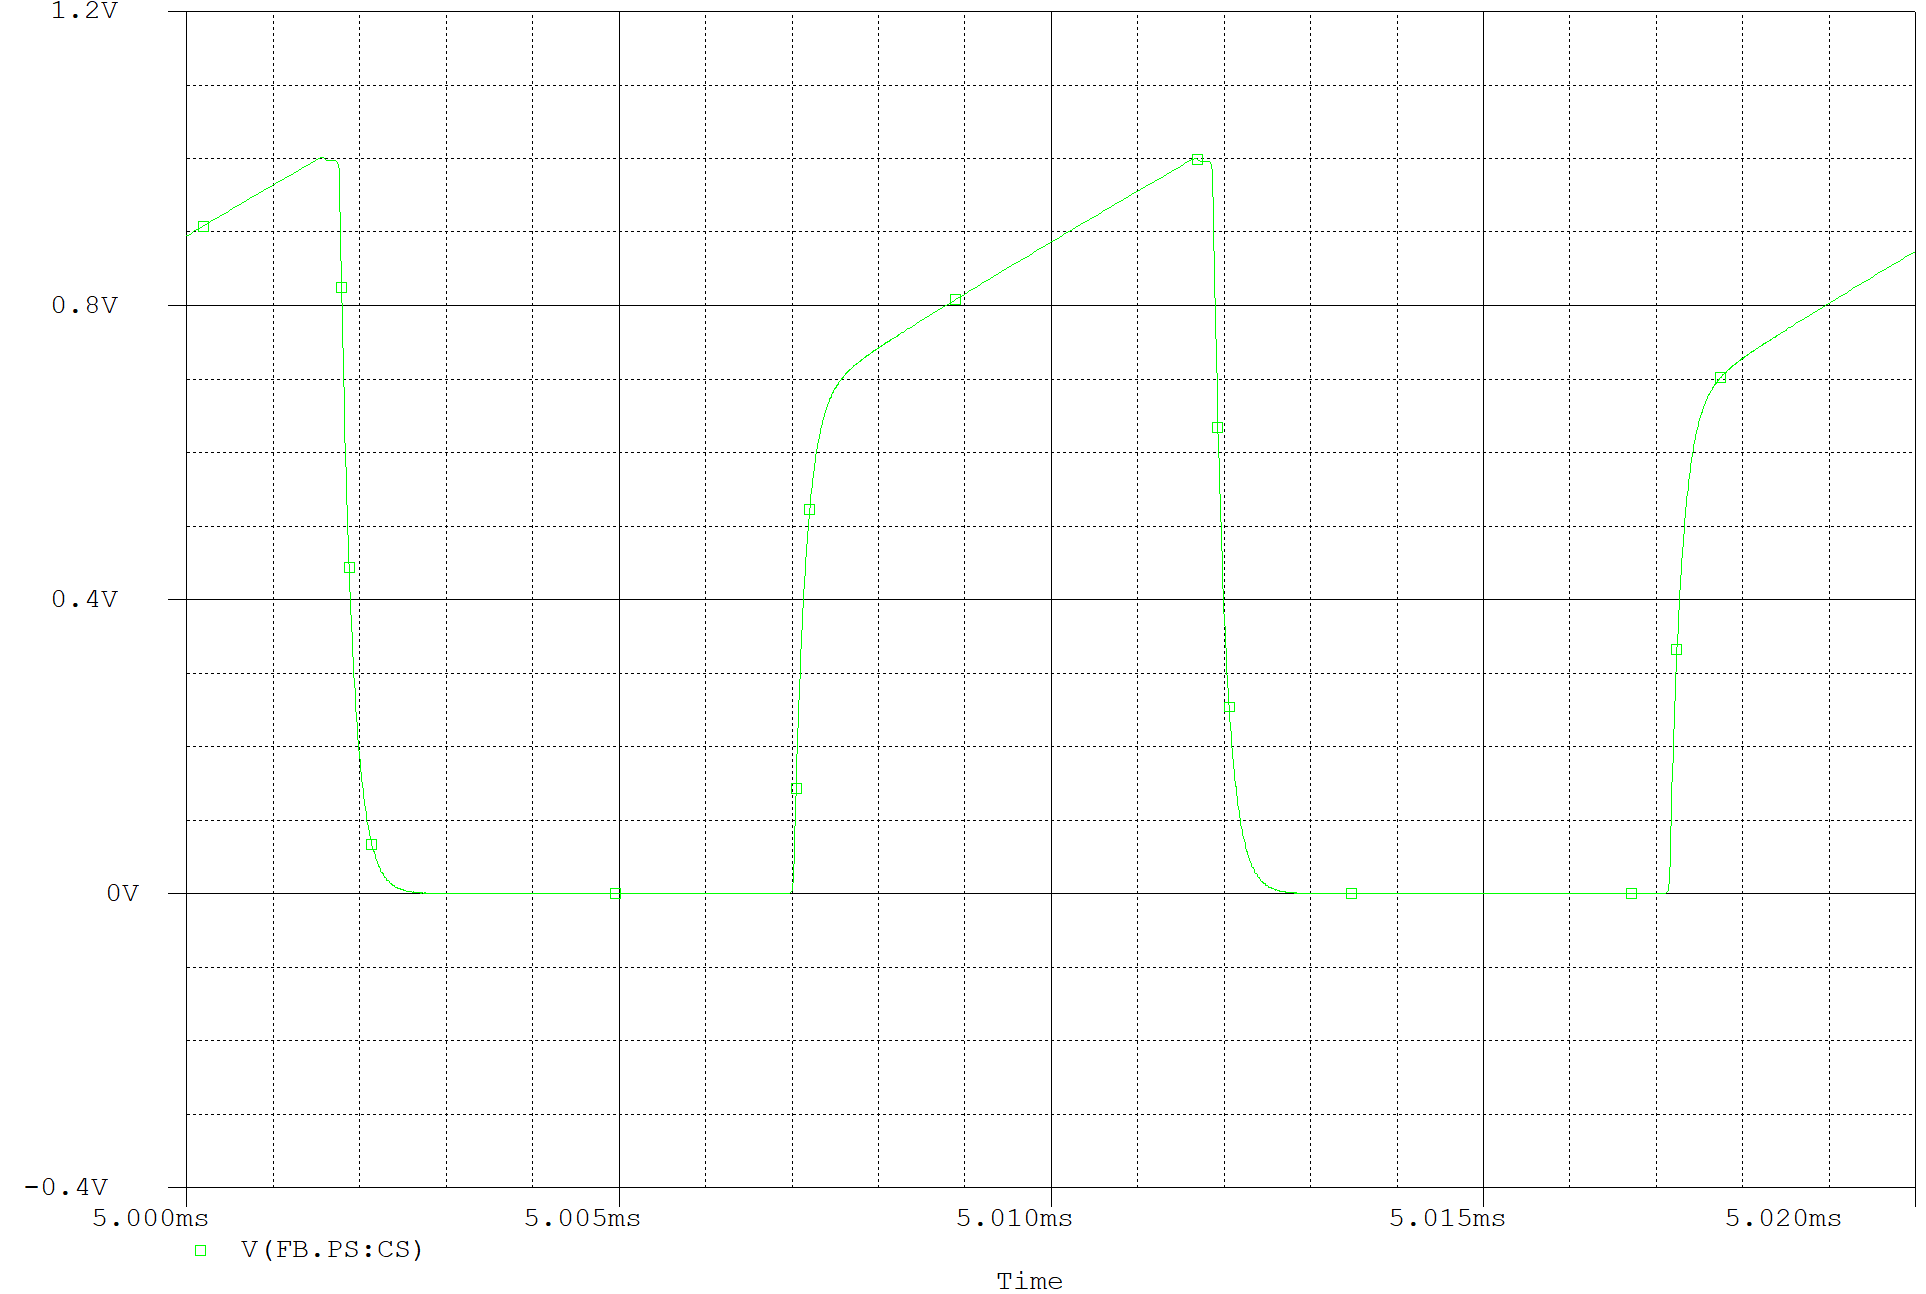
\includegraphics[max width=0.9\linewidth]{/tex/2iteration/billeder/Simulering_PWM_current_sense_M.png}
	\caption{Simulering af current-sense signal efter filtrering}
	\label{fig:Simulering_PWM_current_sense_M}
\end{figure}




\subsection{Constant load}
Ved constant load simuleringen simuleres ved en load på $8.4\ohm$, efter $20ms$ så det sikres, at der ses på den stationære udgang. Indgangsspændingen er sat til 26V.
Første plot af denne simulering ses på figur~\ref{fig: simflycon}. Her ses både strøm og spænding på udgangen.
\begin{figure}[H]
	\center
	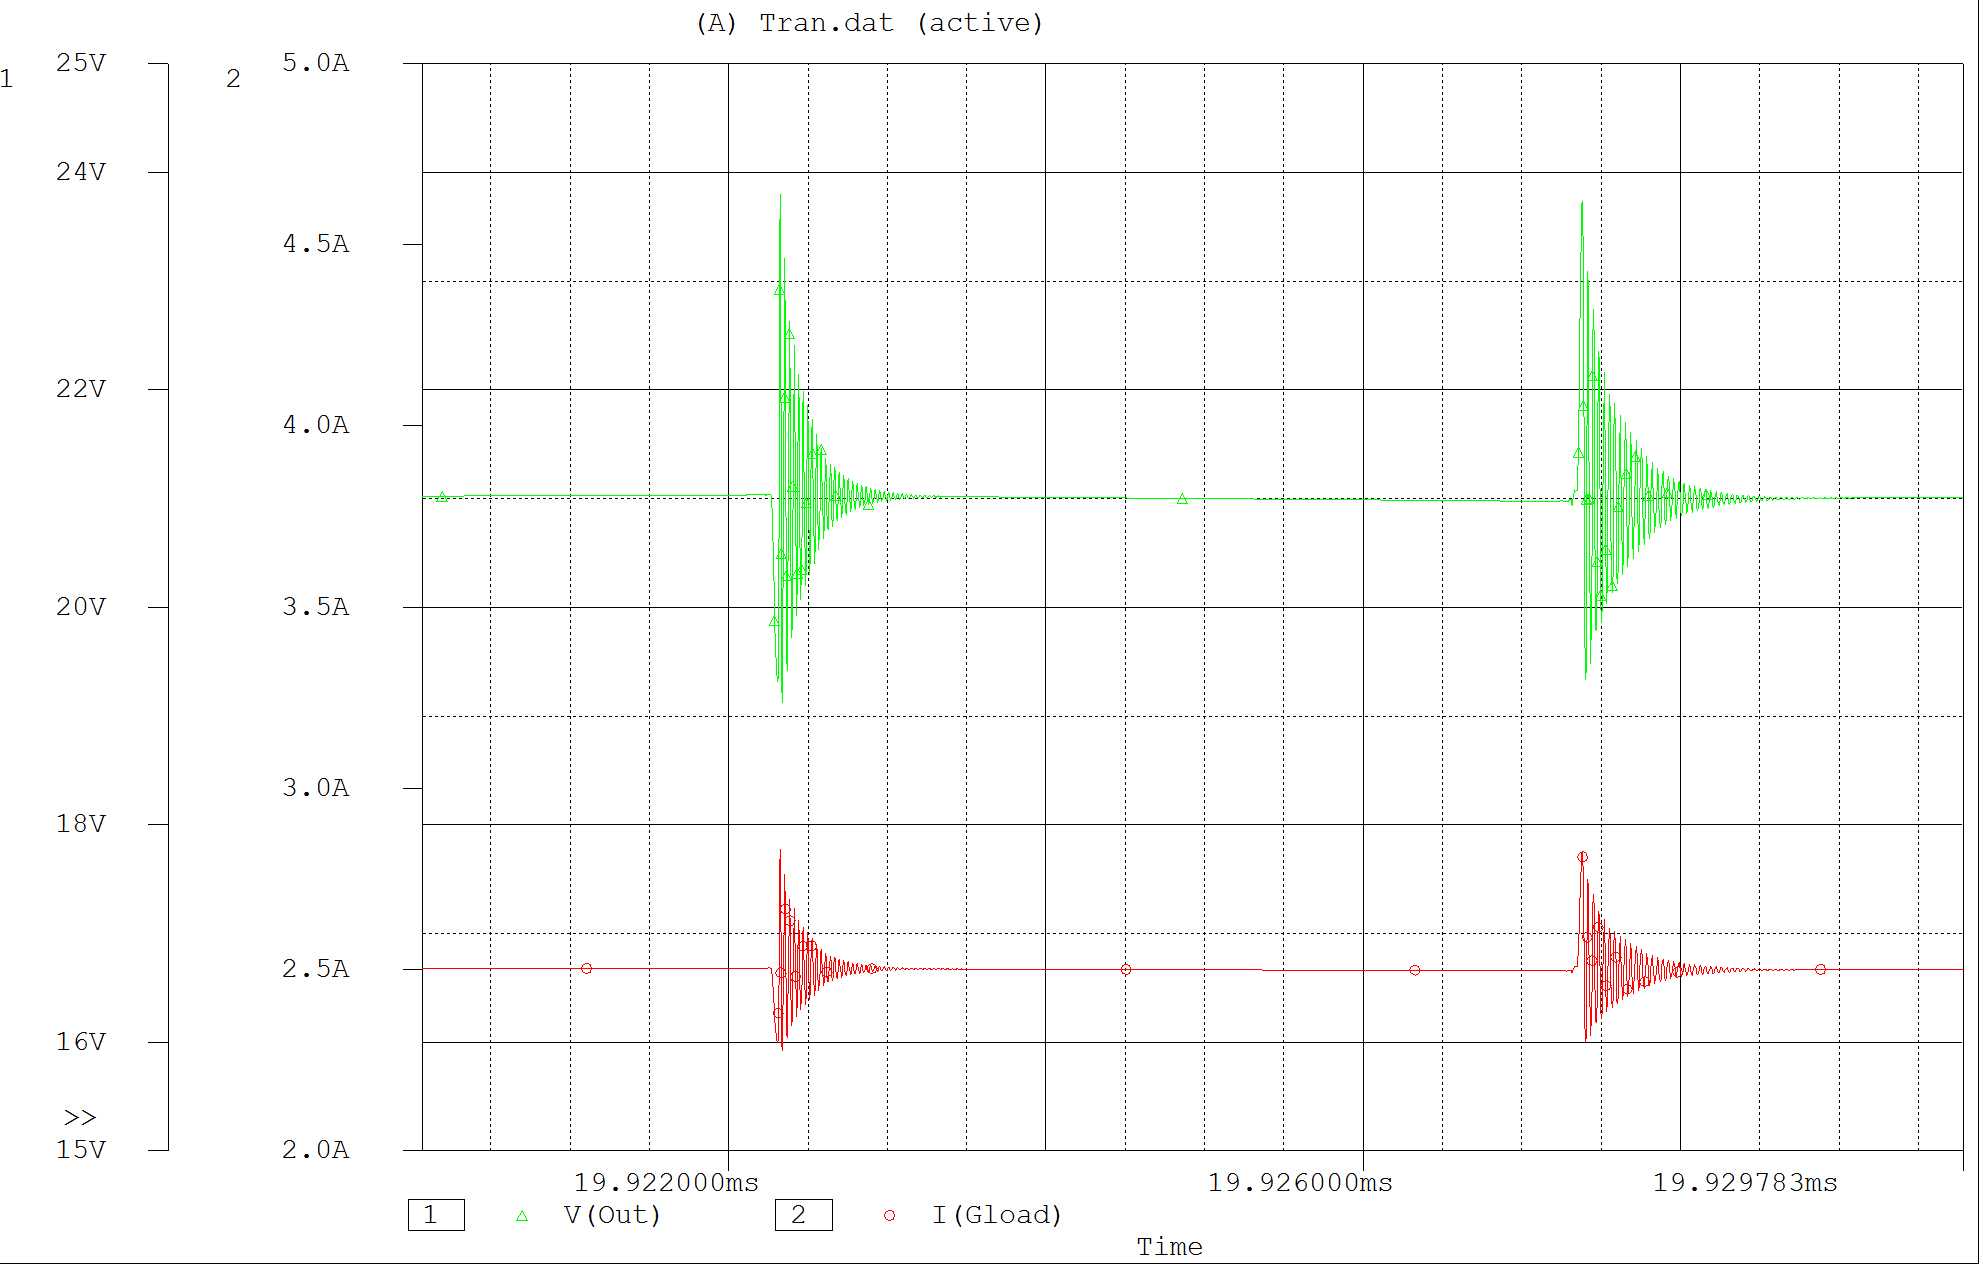
\includegraphics[max width=0.7\linewidth]{/tex/2iteration/billeder/Simudgang.png}
	\caption{Simulering af udgang}
	\label{fig: simudgang}
\end{figure}
Her ses det at spændingen V(out) ligger på 21V, dog med svingninger hver gang der switches. Det ser altså ud til at switching transienter fra MOSFET og diode kommer til syne på udgangen. Det er samme billede for strømmen I(Gload), der ellers ligger på de forventede 2.5A.

På figur~\ref{fig: simMOSdio} ses en spændingsperiode for drain benet på MOSFET'en samt dioden. 
\begin{figure}[H]
	\center
	\includegraphics[max width=0.7\linewidth]{/tex/2iteration/billeder/SIMMOSFETdiode.png}
	\caption{Simulering af spænding over diode og drain ben på MOSFET}
	\label{fig: simMOSdio}
\end{figure}
Det ses, at når transistoren (rød kurve) går off så kommer den tidligere omtalte peakspænding samt den svinger, inden den går til en stationær værdi på ca. 48V, inden MOSFET'en switches on igen. Dette stemmer fint overens med analysen hvor den stationær værdi bør ligge på 21V+26V=47V.
Peak'en er ca. 93V.
Det samme ses for dioden (grøn kurve) at når transistoren er on, vil dioden ikke være i lederetningen, og skal derfor kunne holde til den peak på ca. 80V der ses på grafen. Derudover lægger den sig på en stationær værdi på ca. 46V, hvilket igen stemmer pænt overens med de 47V.

\subsection{Load step}
Ved load steppet kontrolleres det, hvor hurtigt systemet får reguleret ind efter en ny load. Den eneste ændring i schematic'et fra før, ligger i toplaget, som ses på figur~\ref{fig: simloadtop}  
\begin{figure}[H]
	\center
	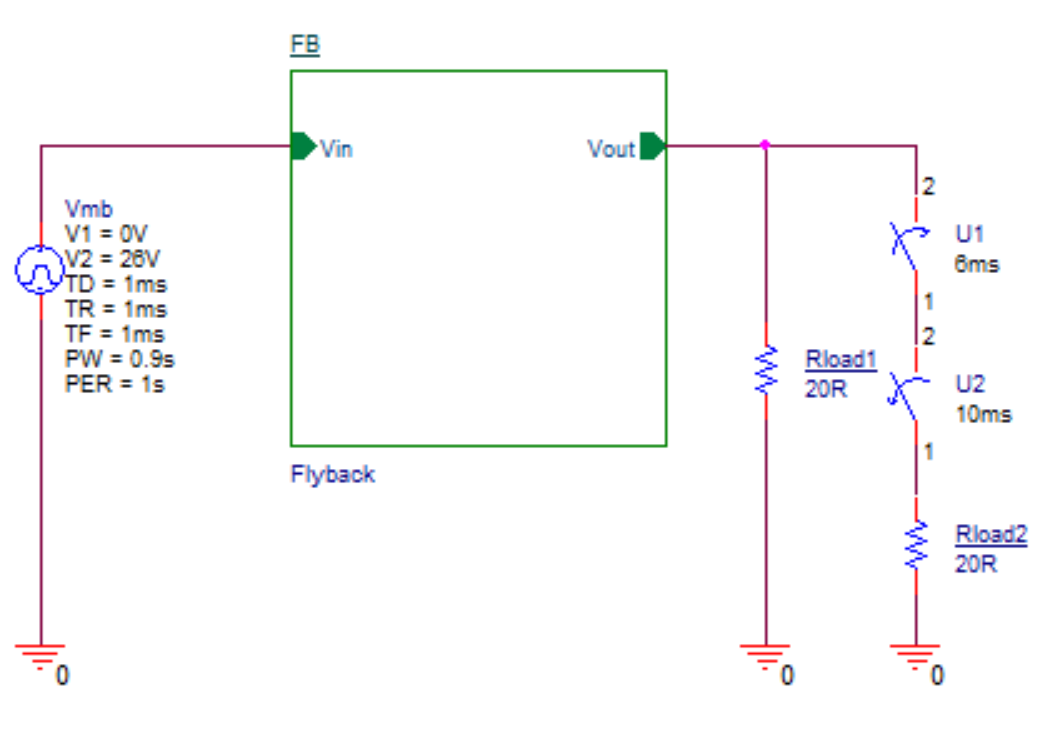
\includegraphics[max width=0.7\linewidth]{/tex/2iteration/billeder/Simloadtop.png}
	\caption{Toplaget for simulering af load step}
	\label{fig: simloadtop}
\end{figure}
Resten af simuleringsblokkene er der ikke ændret ved. Den eneste forskel er i udgangsloaden. Som her består af 2 $20\ohm$ modstande i parallel, hvor den ene sidder for enden af 2 switches. Det gør, at når switchen er off er loaden på $20\ohm$, men når switchen er on er det parallel modstanden af de 2, som vil være 10\ohm. De 2 switches er sat op således, at   



%%% Simulering for optimering af reguleringsloop %%%

\subsection{Gain-fase}
Simuleringen af systemets gain-fase karakteristik, udføres på samme måde som ved 2. iteration. Bode plot for fejlforstærkeren er vist på figur~\ref{fig:Simulering_error_op_amp_3}. Da knækfrekvensen for fejlforstærkeren ligger ved $132\hertz$, og der ikke kan simuleres med frekvenser lavere end $100\hertz$, er det svært at aflæse bode plottet. Det kan dog aflæses, at forstærkningen over $132^\circ$ ligger sig på ca. $8.6\decibel$. Derudover ses det at fasen stiger til $180^\circ$, derfor antages det, at fejlforstærkeren vil bidrage med det forventede faseløft på $90^\circ$. 

\begin{figure}[H]
	\center
	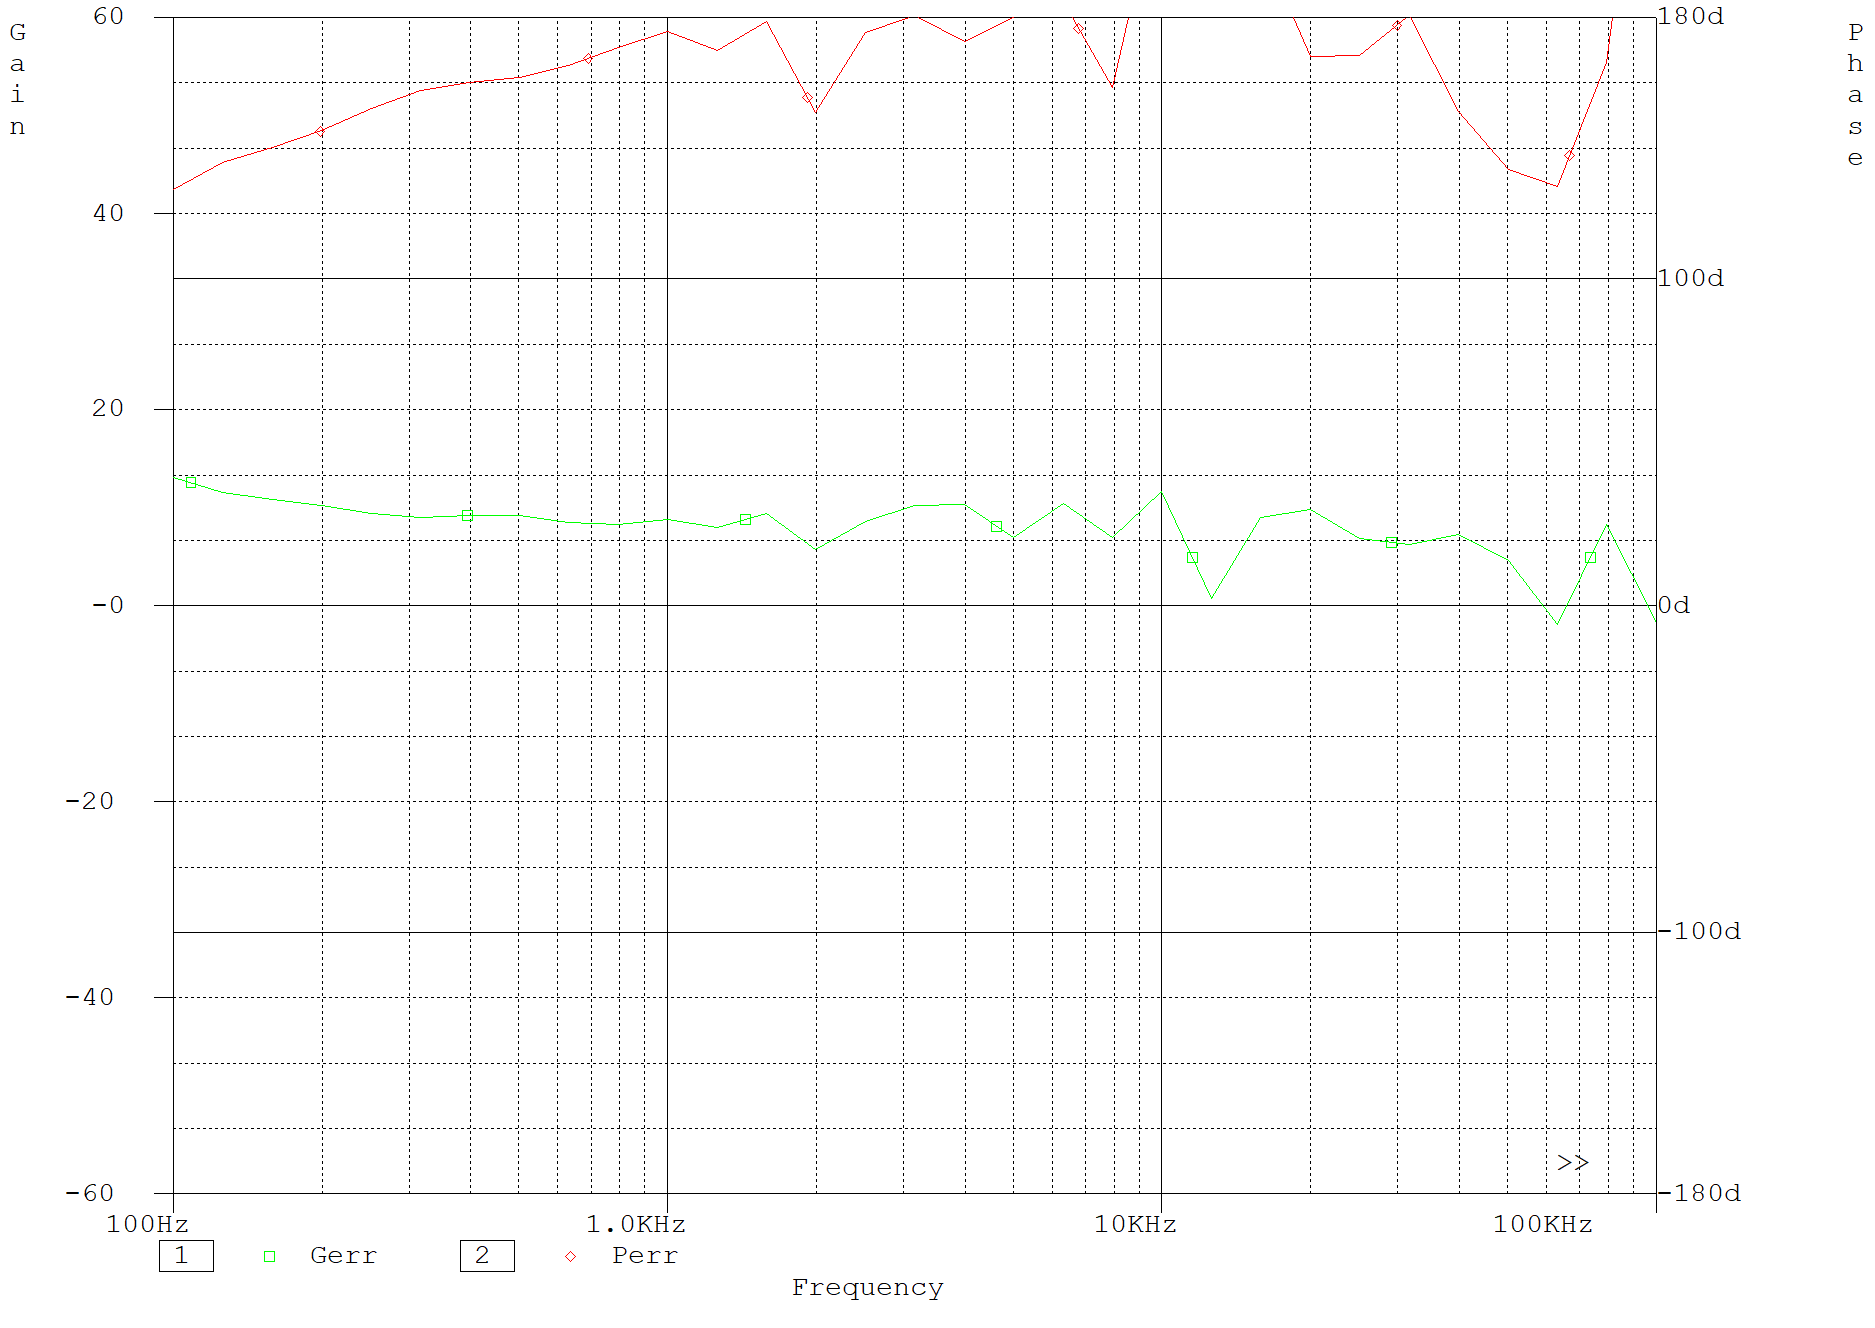
\includegraphics[max width=0.9\linewidth]{/tex/3iteration/billeder/Simulering/Simulering_error_op_amp.PNG}
	\caption{Simulering af fejlforstærkeren}
	\label{fig:Simulering_error_op_amp_3}
\end{figure}

\noindent Bode plottet for det samlede system er vist på figur~\ref{fig:Simulering_total_3}. Selvom simuleringen bliver usikker ved høje frekvenser, sker det så langt oppe i frekvens, at de relevante værdier akkurat kan aflæses. Gain-margin aflæses til ca. $10.2\decibel$, fase-margin aflæses til ca. $73.2^\circ$, og båndbredden aflæses til ca. $3.5k\hertz$. Ift. analysen passer både gain- og fasemargin, mens båndbredden ca. $400\hertz$ lavere end det forventede. 

\begin{figure}[H]
	\center
	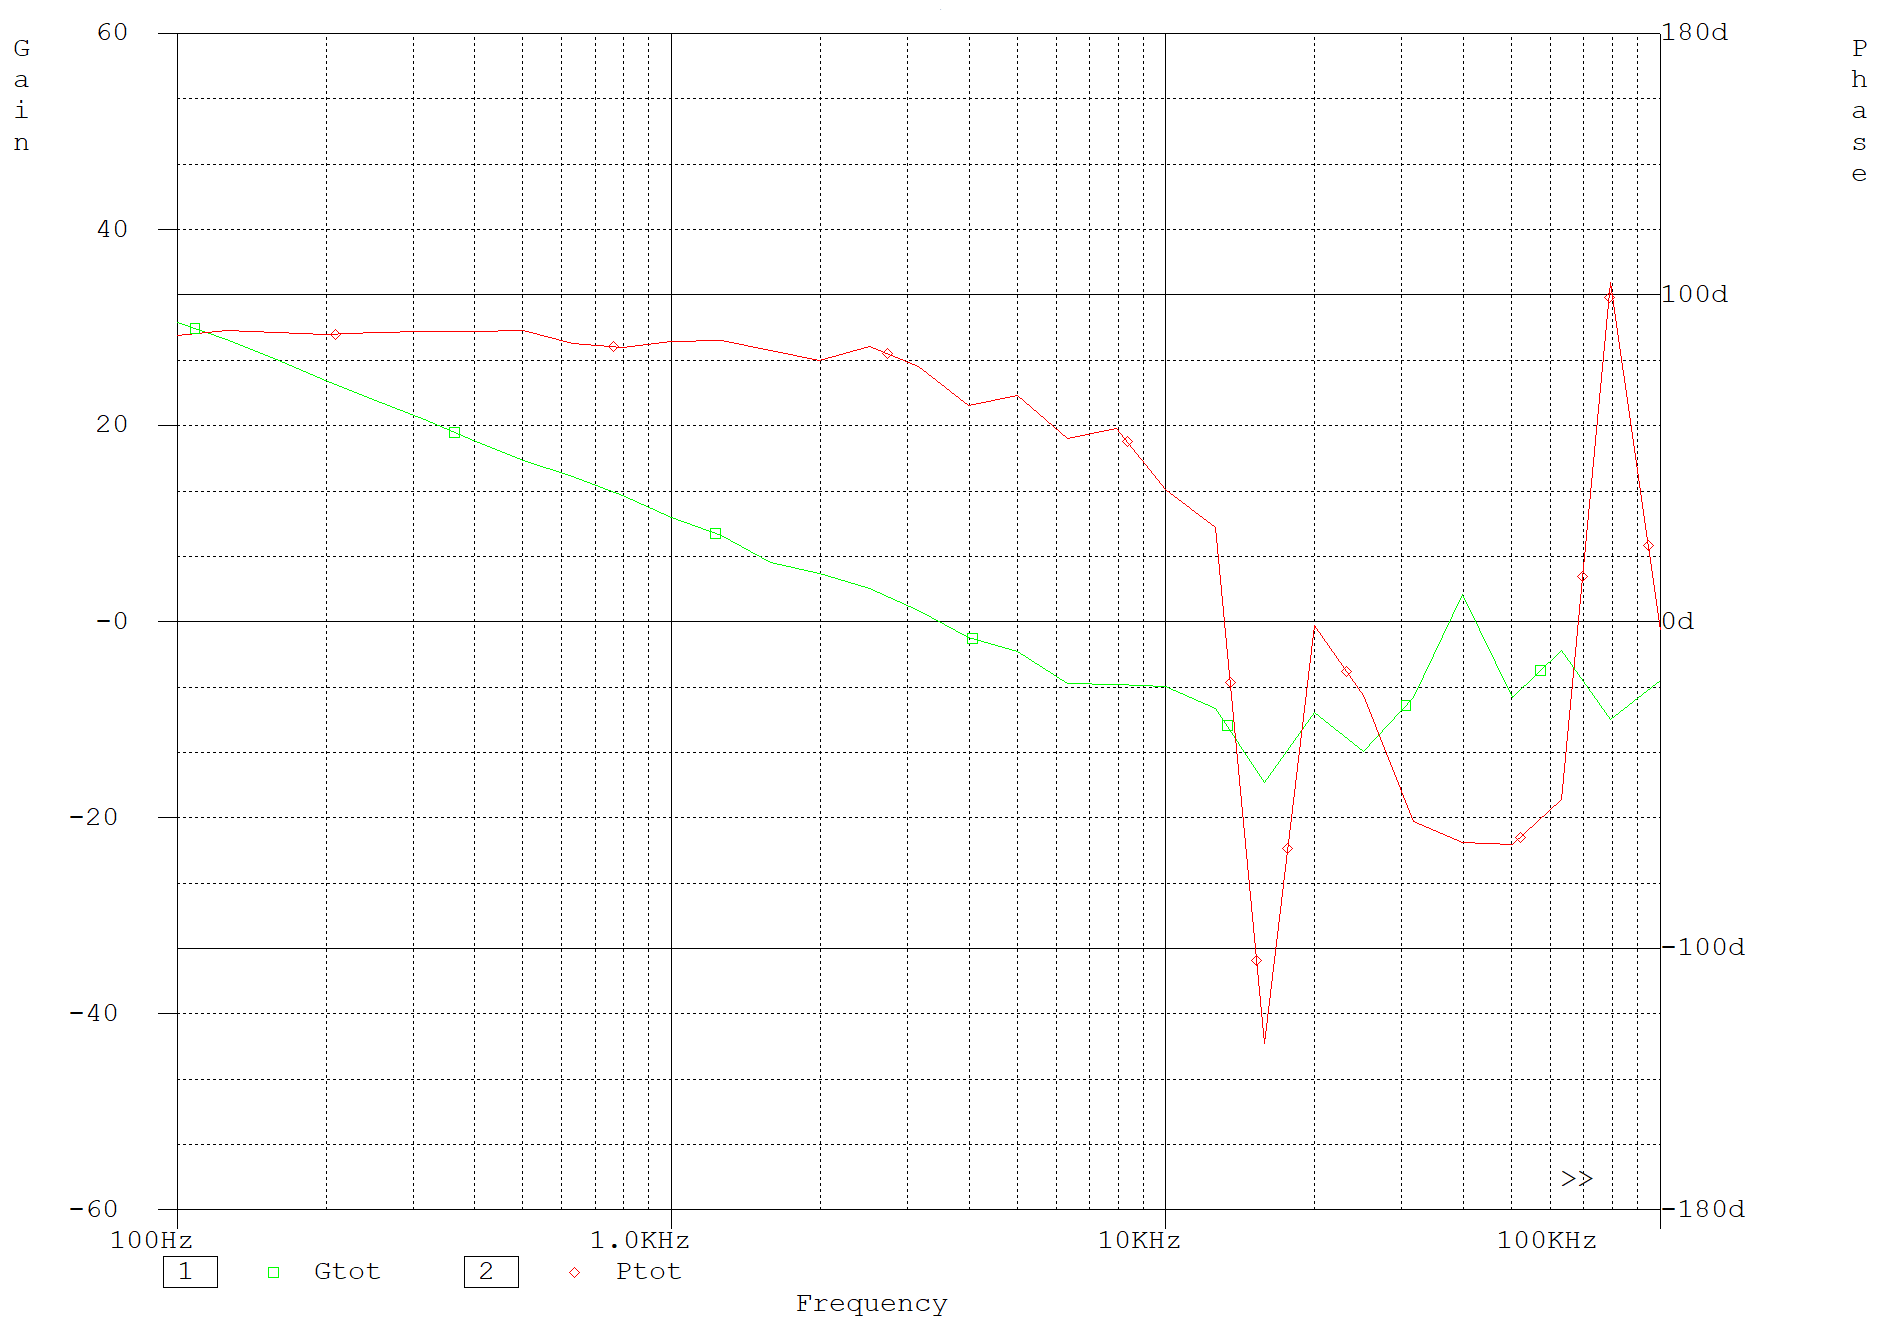
\includegraphics[max width=0.9\linewidth]{/tex/3iteration/billeder/Simulering/Simulering_total.PNG}
	\caption{Simulering af det samlede system}
	\label{fig:Simulering_total_3}
\end{figure}  